%% ------------------------------------------------------------------------- %%
\chapter{Conceitos}
\label{cap:conceitos}

Neste capítulo serão dados algumas definições e conceitos fundamentais sobre
ontologias, além de ferramentas e linguagens relacionadas.

%% ------------------------------------------------------------------------- %%
\section{Ontologias}\index{ontologias!definicao}
\label{sec:definicao}

Ontologias são utilizadas hoje em diversas áreas para organizar a informação.
São encontradas na literatura diversas definições para ontologias, propostas
para aplicação em diferentes áreas de conhecimento e propostas para a construção
de ontologias(metodologias, ferramentas e linguagens).

Uma das definições mais conhecidas para ontologias é apresentada por
\cite{gruber1995toward} que diz que uma ontologia é uma especificação explícita
de uma conceitualização. O termo conceitualização corresponde a uma coleção de
objetos, conceitos e outras entidades que se assume existirem em um domínio e
os relacionamentos entre eles \cite{genesereth1987logical}. Uma conceitualização
é uma visão abstrata e simplificada do mundo que se deseja representar.

Porém essa interpretação por meio de conceitualização é discutida por
\cite{giaretta1995ontologies} quando, afirma que a noção de conceitualização é um
grupo de relações extensionais descrevendo um {\it estado das coisas} particular,
enquanto que a noção que temos em mente é uma relação intensional, nomeando algo
como uma rede conceitual a qual se superpõe a vários possíveis
{\it estados das coisas}.

Com esta abordagem de aspecto intensional \cite{guarino1998formal}, revê a
definição de conceitualização a fim de obter uma interpretação mais clara. Ele
se refere a ontologia como um artefato constituído por um vocabulário usado para
descrever uma certa realidade e um conjunto de fatos explícitos e aceitos
que dizem respeito ao sentido pretendido para as palavras do vocabulário. Este
conjunto de fatos tem a forma da teoria da lógica de primeira ordem, onde as
palavras do vocabulário aparecem como predicados unários ou binários. O
vocabulário formado por predicados lógicos forma a rede conceitual que confere
o caráter intensional às ontologias. A ontologia define as regras que regulam a
combinação entre os termos e as relações.

Uma outra intepretação muito mais simples é dada por
\cite{borst1997construction}. Para ele uma ontologia é uma especificação formal
e explícita de uma conceitualização compartilhada. Nessa definição, "formal"
significa legível para computadores, "especificação explícita" diz respeito a
conceitos, propriedades, relações, funções, restriçṍes, axiomas, explicitamente
definidos; "compartilhado" quer dizer conhecimento consensual; e
"conceitualização" diz respeito a um modelo abstrato de algum fenômeno do mundo
real.

%% ------------------------------------------------------------------------- %%
\section{Tipos de Ontologias}\index{ontologias!tipos de ontologias}
\label{sec:tipos_de_ontologias}

As ontologias podem ser classificadas de diversas formas, porém neste trabalho
será utilizado a classificação quanto a sua função. \cite{guizzardidesenvolvimento}
ainda a define em 5 tipos:

\begin{itemize}
    \item \textit{Ontologias Genéricas}

    São consideradas ontologias mais "gerais" que descrevem conceitos mais
    amplos. Pesquisas enfocando ontologias genéricas procuram construir teorias
    básicas do mundo, de caráter bastante abstrato, aplicáveis a qualquer domínio
    (conhecimento em seu sentido filosófico de categorização e linguística).

    \item \textit{Ontologias de Domínio}

    Descrevem conceitos e vocabulários relacionados a domínios particulares. Este
    é um tipo de ontologia mais comum, que geralmente é utilizada para representar
    um "micro-mundo".

    \item \textit{Ontologias de Tarefas}

    Descrevem tarefas ou atividades genéricas, que podem contribuir na resolução
    de problemas, independente do domínio que ocorrem. Sua principal motivação
    é facilitar a integração dos conhecimentos de tarefa e domínio em uma
    abordagem mais uniforme e consistente, tendo por base o uso de ontologias.

    \item \textit{Ontologias de Aplicação}

    Descrevem conceitos que dependem tanto de um domínio particular quanto de uma
    tarefa específica. Devem ser especializações dos termos das ontologias de
    domínio e de tarefa correspondentes. Estes conceitos normalmente correspondem
    a regras aplicadas a entidades de domínio enquanto executam determinada tarefa.

    \item \textit{Ontologias de Representação}

    Explicam as conceituações que fundamentam os formalismos de representação de
    conhecimento, procurando tornar os compromissos ontológicos embutidos nestes
    formalismos. Um exemplo desta categoria é a ontologia de frames.

\end{itemize}

Neste trabalho será utilizado uma ontologia de domínio.

%% ------------------------------------------------------------------------- %%
\section{Construção de Ontologias}\index{ontologias!construção de ontologias}
\label{sec:construção_de_ontologias}

Primeiramente para a construção de uma ontologia de domínio, é necessário definir
o seu domínio e escopo. Logo em seguida, ainda é necessário escolher uma
metodologia, uma ferramenta e uma linguagem que serão utilizadas para definir a
estrutura da ontologia.

Nem todas as ontologias possuem a mesma estrutura, mas todas possuem pelo menos
um dos elementos básicos abaixo:

\begin{itemize}
    \item \textit{Classes}

    Normalmente organizadas em taxonomias, as classes representam algum tipo de
    integração da ontologia com um determinado domínio.

    \item \textit{Relações}

    Representam o tipo de interação entre os elementos do domínio (classes).

    \item \textit{Axiomas}

    São utilizados para modelar sentenças consideradas sempre verdadeiras.

    \item \textit{Instâncias}

    São utilizadas para representar elementos específicos, isto é, os próprios
    dados da ontologia.
\end{itemize}

%% ------------------------------------------------------------------------- %%
\section{Metodologia para Construção de Ontologias}
\index{ontologias!metodologias para construção de ontologias}
\label{sec:metodologias_para_construcao_de_ontologias}

As metodologias para construção de ontologias tem por objetivo organizar e definir
um padrão para sua construção. O problema é que ainda não estão suficientemente
maduras e não conseguem demonstrar um processo realmente estruturado a ponto de
ser considerado um padrão de fato. Por isso, \cite{guizzardidesenvolvimento}
sugere uma abordagem sistemática para a sua construção. Essa metodologia é
composta por 6 fases.

A figura abaixo demonstra o diagrama de atividade que ilustra esta metodologia.

\begin{figure}[!h]
  \centering
  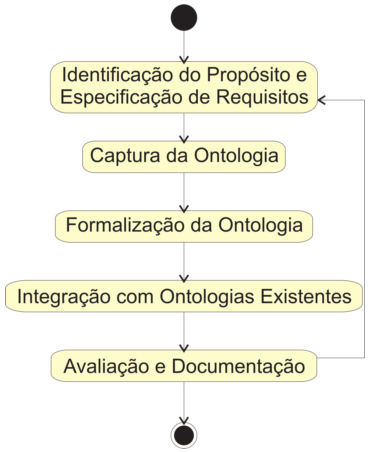
\includegraphics[width=.40\textwidth]{fig_metodologia_diagrama}
  \caption{Diagrama de atividades da metologia proposta por
    \cite{guizzardidesenvolvimento}. Fonte da imagem \cite{morais2007ontologias}.
  }
  \label{fig:diagrama_metodologia}
\end{figure}

\begin{itemize}
    \item \textit{Identificação de Propósito e Especificação de Requisítos}

    Tem o objetivo de identificar a competência da ontologia, ou seja, seus usos
    e propósitos, e para atingir isso limita-se no que é relevante para a ontologia
    e o que não é. Nesta fase também identificam-se potenciais usuários da ontologia,
    e o contexto base que motivou sua construção.

    Após a definição das competências, ainda é preciso especificar algumas
    questões que a ontologia deve ser capaz de responder. Essa especificação
    envolve a descrição do propósito e dos usos da ontologia e servem também para
    justificar a existência da ontologia e para futuras avaliações da mesma.

    \item \textit{Captura da Ontologia}

    Esta é considerada a fase mais importante, o seu objetivo é capturar o
    conjunto de elementos de um domínio que podem ser representados em uma
    ontologia, com base nas questões de competência relacionadas a esta.

    Na captura é feita a identificação dos conceitos (classes), seus
    relacionamentos e todos os demais elementos exigidos na construção de uma
    ontologia, como: axiomas, instâncias e propriedades.

    Os conceitos, suas propriedades e relacionamentos, formam a base de qualquer
    ontologia. Entretanto para definir a semântica de seus termos devem ser
    construídos os axiomas, que são utilizados para modelar sentenças sempre
    verdadeiras. Na prática axiomas especificam definições em linguagem natural,
    mas também podem ser especificados através de lógica de primeira ordem
    \cite{falbo1998integracao}.

    \item \textit{Formalização da Ontologia}

    A formalização de uma ontologia diz respeito a especifica-la por meio de uma
    linguagem. Embora uma ontologia possa ser representada por meio de qualquer
    linguagem, ou seja, formal ou não formal, a linguagem formal por ser baseada
    em um modelo matemático permite que sejam realizadas pressuposições
    implícitas e com isso testada com maior precisão e facilidade.

    \item \textit{Integração com Ontologias Existentes}

    \cite{falbo1998integracao} destaca que na fase de captura e formalização,
    pode aparecer a necessidade de integrar a ontologia que se esta criando com
    uma outra já existente, e isto deve ser incentivado pois é uma boa prática
    aproveitar conceituações previamente estabelecidas em outras ontologias,
    isso reduz o trabalho de ter que reinventar todos os conceitos novamente.

    \item \textit{Avaliação}

    \cite{guizzardidesenvolvimento} sugere que esta fase seja executada em
    conjunto com as fases de captura e formalização. Esta fase visa garantir
    que os requisítos definidos antes da construção da ontologia foram atendidos.
    Para isso, pode-se considerar alguns critérios, como: clareza, coerência,
    extensibilidade e compromissos ontológicos mínimos.

    \item \textit{Documentação}

    Todo o processo de construção da ontologia deve ser documentado, e esta etapa
    inclui os propósitos, requisitos e cenários de motivação, as descrições
    textuais da conceituação, a ontologia formal e os critérios de projeto
    adotados.
\end{itemize}

%% ------------------------------------------------------------------------- %%
\section{Ferramentas para Construção de Ontologias}
\index{ontologias!ferramentas para construção de ontologias}
\label{sec:ferramentas_para_construcao_de_ontologias}

O processo de construção de uma ontologia é uma tarefa custosa e complexa, por
isso existem algumas ferramentas e APIs que permitem desde manipulação de
ontologias, consultas até integração com outras aplicações.

A ferramenta que será utilizada neste trabalho é o Protégé (versåo 4),
veja a figura \ref{fig:fig_protege_apresentacao}. O Protégé foi criado
no Centro de Pesquisa em Informática Biomédica da Universidade de Stanford
\cite{protege}, possui código aberto e por meio dele é possível criar e
manipular ontologias. Outra característica muito interessante do Protégé,
é permitir a escalabilidade e extensibilidade através de uma arquitetura de
plugins.

\begin{figure}[!h]
  \centering
  \includegraphics[width=.40\textwidth]{fig_protege_apresentacao}
  \caption{Protége}
  \label{fig:fig_protege_apresentacao}
\end{figure}

%% ------------------------------------------------------------------------- %%
\section{Padrões para Representação de Ontologias}
\index{ontologias!padrões para representação de ontologias}
\label{sec:padroes_para_representacao_de_ontologias}

Muitas linguagens utilizadas para representção de ontologias são baseadas na
tecnologia XML (Extensible Markup Language), mas também existem outras como
Turtle e N3.

\subsection{RDF}
\index{ontologias!rdf}
\label{sec:rdf}

Desenvolvido pelo W3C (World Wide Web Consortium), por meio da utilização de
redes semânticas o RDF (Resource Description Framwork) tem como objetivo a
representação do conhecimento. Embora não seja uma linguagem muito expressiva,
permite a representação de conceitos, taxonomias de conceitos e relações binárias \cite{lassila1999resource}.

A estrutura básica do RDF é um grafo dirigido e etiquetado, onde as arestas
dão nome a ligação entre dois recursos, que são representados pelos nós do grafo.
A formalização desse grafo é um conjunto de triplas, composto por sujeito,
predicado e objeto.

A figura \ref{fig:fig_tripla_rdf} apresenta uma trilpa em RDF.

\begin{figure}[!h]
  \centering
  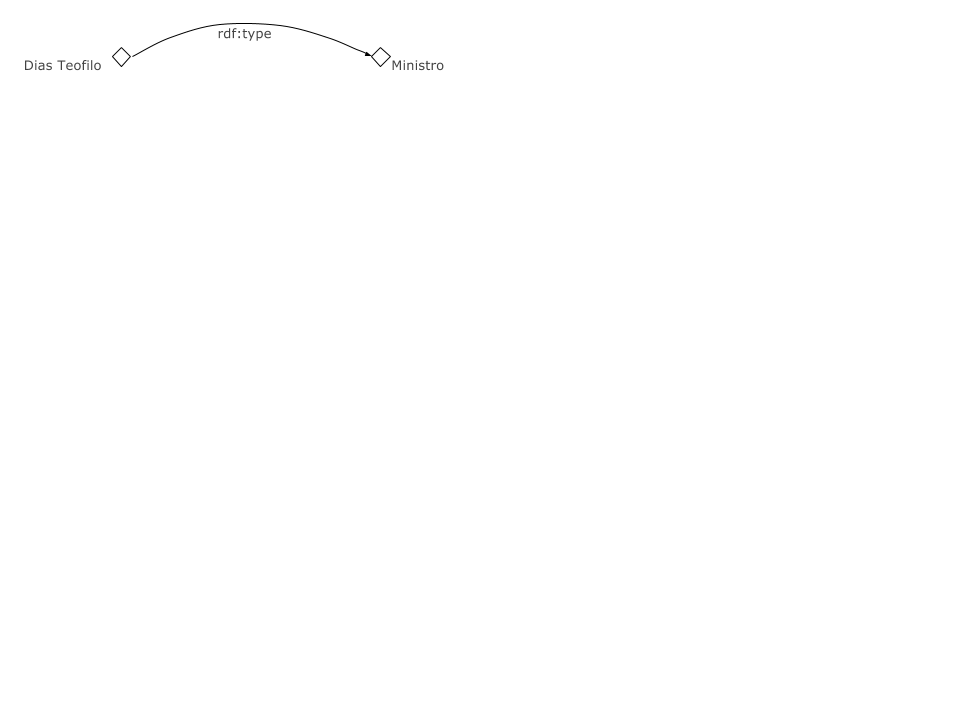
\includegraphics[width=.40\textwidth]{fig_tripla_rdf}
  \caption{Exemplo de tripla em RDF}
  \label{fig:fig_tripla_rdf}
\end{figure}

\vskip 0.6cm

Fragmento de código em RDF:

\vskip 0.25cm

\lstset{language=XML,basicstyle=\ttfamily,breaklines=true}
\begin{lstlisting}
<NamedIndividual rdf:about="&ontoSTF;DiasToffoli">
    <rdf:type rdf:resource="&ontoSTF;Ministro"/>
</NamedIndividual>
\end{lstlisting}

\vskip 0.25cm

Os recursos no RDF fazem referência a qualquer elemento, abstrato ou não, eles
podem também receber a denominação de entidades e devem sempre estar associados
por um identificador, ous seja, uma URI que seja capaz de fornecer identificação
única e global. A propriedade é um tipo especial de recurso dentro do RDF, que
descreve relações. Isso facilita a utilização em um ambiente de conhecimento
distribuído como a internet.

Apesar do RDF ter sido publicado pelo W3C em XML, o mesmo pode utilizar outras
linguagens como as mencionadas acima, pois em camparação com o XML, elas não
apresentam nenhuma diferença na capacidade de representação.

\subsection{RDFs}
\index{ontologias!rdfs}
\label{sec:rdfs}

O RDFs (Reource Description Framework Schema) foi criado com o intuito de
expandir a expressividade semântica das
descrições criadas em RDF, pois embora o RDF seja muito flexível e expressivo,
o que torna possível dizer qualquer coisa sobre qualquer coisa
\cite{hebeler2011semantic}, por outro lado ele não consegue dar suporte para
a especificação de significados semânticos.

O RDFs fornece mecanismos para descrever grupos de recursos relacionados e a
relação entre esses recursos. Uma classes em RDFs se
assemelha a uma classe do paradigma de programação de orientação a objetos, pois
é possível descrever hierarquias de especialização/generalização de classes e
criar objetos como instâncias dessas classes.

As principais classes utilizadas no RDFs, são:

\begin{itemize}
    \item \textbf{rdfs:Resource}, é a classe de todos os recursos;

    \item \textbf{rdfs:Class}, é a classe de todas as classes;

    \item \textbf{rdfs:Literal}, é a classe de todos literais (string);

    \item \textbf{rdfs:Property}, é a classe de todas as propriedades;

    \item \textbf{rdfs:Statement}, é a classe de todas as declarações
    representadas;

    Alguns dos termos presentes na codificação das relações semânticas em RDFs
    são:

    \item \textbf{rdfs:type}, que relaciona um recurso a uma classe, declarando-o
    como uma instância daquela classe;

    \item \textbf{rdfs:subClassOf}, é quem relaciona uma classe com algumas de
    suas superclasses;

    \item \textbf{rdfs:subPropertyOf}, que relaciona uma propriedade com algumas
    de suas super propriedades;

    O RDFs ainda da suporte para algumas restrições semânticas das propriedades,
    como:

    \item \textbf{rdfs:domain}, que especifica um domínio de uma dada propriedade,
    ditando que qualquer recurso que tem essa propriedade é uma instância das
    classes referenciadas nesse domínio;

    \item \textbf{rdfs:range}, que especifica o alcance da propriedade;
\end{itemize}

%%TODO incluir imagem e XML com exemplo de RDFs

\subsection{OWL}
\index{ontologias!owl}
\label{sec:owl}

O OWL é uma extensão do vocabulário RDFs, que foi criado com o intuito de dar
suporte a recursos que permitem a construção de ontologias mais complexas, voltadas
para a web. Ela introduziu novas restrições na estrutura de representação do RDF,
com o objetivo de tornar as inferências computacionais decidíveis.

Dentre as várias características que a linguagem OWL apresenta, as mais
relevantes para este trabalho são:

\begin{itemize}

    \item \textit{Indivíduos}

    Os indivíduos representam o objeto no domínio de interesse. Como não
    utiliza o \textit{Unique Name Assumption}, o OWL permite que dois nomes
    diferentes referêncie o mesmo indíviduo. Exemplo, \textit{Queen Elizabeth}
    (Rainha Elizabeth) e \textit{Elizabeth Windsor} podem ser referências ao
    mesmo indíviduo. No OWL deve ser declarado explicitamente que os indíviduos
    são os mesmos, ou diferentes uns dos outros \cite{horridge2004practical}.

    \item \textit{Propriedades}

    As propriedades são relações binárias entre os indivíduos, esta relação pode
    ser entre indivíduos do tipo propriedade primitiva
    (\textit{DataType Property}), ou outro indivíduo do tipo propriedade objeto
    (\textit{Object Property}) \cite{horridge2004practical}. Por exemplo, a
    propriedade \textit{hasSibling} liga o indivíduo Mathew ao indivíduo Gemma,
    ou a propriedade \textit{livesIn} pode ligar o indivíduo Mathew ao indivíduo
    England. A figura \ref{fig:fig_owl_1} mostra os exemplos de propriedades que ligam indivíduos.

    \begin{figure}[!h]
      \centering
      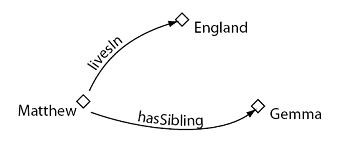
\includegraphics[width=.40\textwidth]{fig_owl_1}
      \caption{Relação entre propriedades e indivíduos}
      \label{fig:fig_owl_1}
    \end{figure}

    As propriedades também podem ser inversas. Por exemplo, a propriedade
    inversa de hasParent é hasChild.

    \begin{figure}[!h]
      \centering
      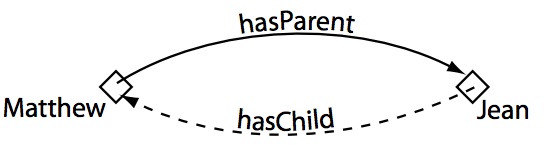
\includegraphics[width=.40\textwidth]{fig_owl_2}
      \caption{Relação inversa}
      \label{fig:fig_owl_2}
    \end{figure}

    \vskip 4cm

    As propriedades podem limitar-se a um único valor, estas são chamadas de
    propriedades funcionais. Na figura abaixo demonstra que Jean só pode ter
    uma única mãe biológica (\textit{hasBirthMother}).

    \begin{figure}[!h]
      \centering
      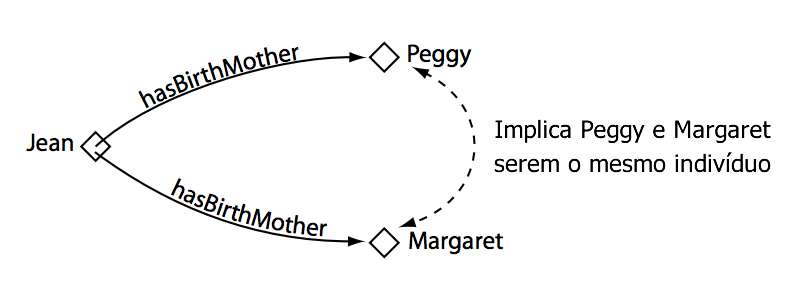
\includegraphics[width=.40\textwidth]{fig_owl_3}
      \caption{Relação funcional}
      \label{fig:fig_owl_3}
    \end{figure}

    \vskip 0.6cm

    \textit{Transitiva}: se a propriedade \textbf{p} é transitiva, e esta
    propriedade relaciona o indivíduo \textbf{a} com o indivíduo \textbf{b}, e a
    mesma propriedade relaciona o indivíduo \textbf{b} com o indivíduo \textbf{c},
    então pode-se inferir que o indivíduo \textbf{a} esta relacionado com o
    indivíduo \textbf{c} através da propriedade \textbf{p}. A figura demonstra
    o exemplo de transitividade.

    \begin{figure}[!h]
      \centering
      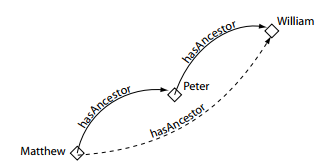
\includegraphics[width=.40\textwidth]{fig_owl_4}
      \caption{Relação transitiva}
      \label{fig:fig_owl_4}
    \end{figure}

    \vskip 0.6cm

    \textit{Simétrica}: se a propriedade \textbf{p} é simétrica, e esta
    propriedade relaciona o indivíduo \textbf{a} com o indivíduo \textbf{b} então
    o indivíduo \textbf{b} também está relacionado com o indivíduo \textbf{a} pela
    propriedade \textbf{p}. A figura demonstra um exemplo de propriedade simétrica.

    \begin{figure}[!h]
      \centering
      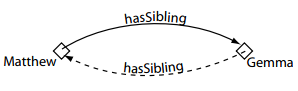
\includegraphics[width=.40\textwidth]{fig_owl_5}
      \caption{Relação simétrica}
      \label{fig:fig_owl_5}
    \end{figure}

    \vskip 0.6cm
\end{itemize}

\section{SPARQL}
\index{ontologias!sparql}
\label{sec:sparql}

O SPARQL é uma linguagem de consulta que é capaz de recuperar e manipular
informações armazenadas no formato RDF. Por ser uma linguagem orientado a dados,
isso implica que não existe nenhum motor de inferência na própria linguagem.

As consultas no SPARQL são baseadas em triplas RDF, ou seja, compostas por
\textit{sujeito}, \textit{predicado} e \textit{objeto}.

\lstset{language=SQL,basicstyle=\ttfamily,breaklines=true}
\begin{lstlisting}
PREFIX p:<URI>
ASK {
        p:joao p:hasParent "joaozinho"
    }
\end{lstlisting}

\vskip 0.6cm

Na consulta acima <URI> é a URI, o identificador de recurso da ontologia.
PREFIX é a palavra chave  que declara p como um \textit{alias} da URI. joao é o
sujeito, hasParent é o predicado e joaozinho é o objeto.

\textbf{Tipos de consultas}

Os tipos de consultas que o SPARQL provê são \cite{beckett2006sparql}:

\begin{itemize}

    \item \textbf{SELECT}: É utilizado para extrair valores brutos de uma base
    RDF, os resultado são apresentados em uma tabela

    \item \textbf{CONSTRUCT}: É utilizado para extrair informações de uma base
    RDF e transformar o resultado em um RDF válido

    \item \textbf{DESCRIBE}: É utilizado para extrair um gráfico de uma base
    RDF

    \item \textbf{ASK}: É utilizado para fornecer um resultado simples em formato
    booleano de uma base RDF

\end{itemize}

\section{OBDA}
\index{ontologias!obda}
\label{sec:obda}

O OBDA (Ontology-based data access) \cite{bagosi2014ontop} é o paradigma de acesso
de dados por meio de uma camada semântica. Usualmente esta camada é expressa na
forma de uma ontologia em RDF/RDFs ou OWL e o dado é armazenado em uma base de
dados relacional. Os termos na camada semântica são mapeados para a camada de
dados utilizando um mapeamento que associa cada elemento da camada semântica com
uma consulta correspondente para a base de dados.

Após este mapeamento é gerado internamente um grafo virtual que permite consultas
utilizando linguagens RDF como SPARQL.

Formalmente, um sistema OBDA é uma tripla \cite{bagosi2014ontop} \textbf{O}
= <\textbf{T},\textbf{S},\textbf{M}>, onde:

\begin{itemize}

    \item \textbf{T} é o nível desejado de uma ontologia

    \item \textbf{S} é a base de dados relacional representando a fonte de dados

    \item \textbf{M} é o conjunto de asserções de mapeamentos, cada um na forma

\end{itemize}

\begin{center}
    $\Phi$(\textbf{x}) $\leftarrow$ $\Psi$(\textbf{x})
\end{center}

onde

\begin{itemize}

    \item $\Phi$(\textbf{x}) é uma consulta sobre \textbf{S}, e como
    resultado retorna tuplas \textbf{x}

    \item $\Psi$(\textbf{x}) é uma consulta sobre \textbf{T} onde as
    variáveis livres são \textbf{x}

\end{itemize}

A principal função de uma sistema OBDA é a execução de consultas. Uma descrição
do processo de transformação de consultas (tipicamente do SPARQL para SQL)
realizado por um sistema OBDA é mostrado na figura \ref{fig:fig_obda_1}.

\begin{figure}[!h]
  \centering
  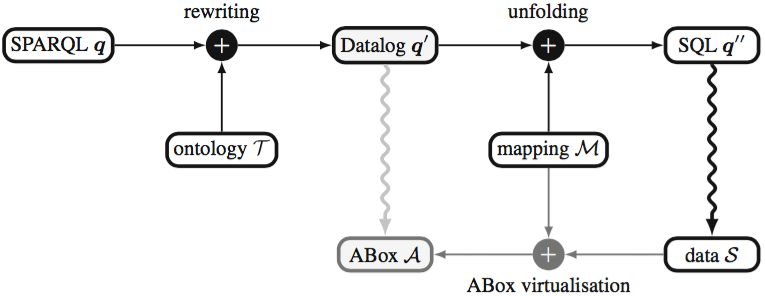
\includegraphics[width=.40\textwidth]{fig_obda_1}
  \caption{Processo de transformação de consulta em um sistema OBDA}
  \label{fig:fig_obda_1}
\end{figure}

\subsection{O Framework Ontop}
\index{ontologias!ontop}
\label{sec:ontop}

O Ontop é um framework de código aberto para o OBDA, liberado sob a licença
Apache e desenvolvido pela Free University of Bozen-Bolzano. Ele suporta todas as
recomendações do W3C \cite{bagosi2014ontop}: OWL, R2RML, SPARQL, SWRL e SPARQL
OWL 2 QL. Além disso as maiores base de dados tanto comerciais quanto livres são
suportadas. Para cada componente do sistema OBDA, o Ontop suporta uma série de padrões:

\begin{itemize}

    \item \textbf{Mapeamento}: O Ontop suporte duas linguagens de mapeamento:
    (1) uma própria e nativa do próprio Ontop, a qual é de fácil aprendizado
    e utilização e (2) a (RDB2RDF mapping language) R2RML que é uma recomendação
    do W3C.

    \item \textbf{Ontologia)}: O Ontop tem suporte completo ao OWL2 QL

    \item \textbf{Base de Dados)}: O Ontop suporta todas as bases de dados que
    implementam SQL99. Isto inclui a maioria das bases de dados relacionais como:
    PostgreSQL, MySQL, H2, DB2, Oracle a MS SQL Server.

    \item \textbf{Consulta)}: O Ontop suporta todas as funcionalidades do SPARQL
    1.0 e SPARQL OWL QL do SPARQL 1.1

\end{itemize}

O framework Ontop pode ser utilizado como:

\begin{itemize}

    \item \textit{plugin para o Protégé 4} que provê uma interface gráfica para
    edição, mapeamento e execução de consultas SPARQL,

    \item \textit{biblioteca java} que implementa tanto a API OWL e API Sesame

\end{itemize}

Neste trabalho iremos utilizar o Ontop em forma de plugin para o Prétege 4.
